\clearpage

\lehead[]{\sf\hspace*{-2.00cm}\textcolor{white}{\colorbox{lightblue}{\parbox[c][0.70cm][b]{1.60cm}{
\makebox[1.60cm][r]{\thechapter}\\ \makebox[1.60cm][r]{ÜBUNG}}}}\hspace{0.17cm}\textcolor{lightblue}{\chaptertitle}}
\rohead[]{\textcolor{lightblue}{\chaptertitle}\sf\hspace*{0.17cm}\textcolor{white}{\colorbox{lightblue}{\parbox[c][0.70cm][b]{1.60cm}{\thechapter\\
ÜBUNG}}}\hspace{-2.00cm}}
%\chead[]{}
\rehead[]{\textcolor{lightblue}{AvHG, Inf, My}}
\lohead[]{\textcolor{lightblue}{AvHG, Inf, My}}

\section{Farben und Zufallszahlen -- Übungen}

\subsection{Aufgabe 1: Wald}

\begin{compactenum}[a)]
\item Erzeuge ein Anwendungsfenster mit einer Breite von 800 und einer Höhe von
700 Pixeln. Das Anwendungsfenster soll einen hellbraunen oder beigen
Hintergrund erhalten. Die Hintergrundfarbe musst du selber mischen.
\item Programmiere eine Methode \lstinline|baum()|, die einen Baum an einer
bestimmten Stelle des Fensters malen kann. Die Methode erhält das
\myClass{Graphics}-Objekt und die x- und y-Koordinate der linken oberen Ecke
übergeben, die in der Zeichnung unten mit einem Kreuz markiert ist. Zeichne die
Baumkrone als ausgefüllten dunkelgrünen Kreis von 50 Pixeln Durchmesser und den
Baumstamm als ausgefülltes braunes Rechteck von 50 Pixeln Höhe und 10 Pixeln
Breite.
\item Erzeuge mit Hilfe der Methode aus Teil b) drei einzelne Bäume an den
 Positionen (20,80), (100,100) und (200,50).
\item Erzeuge mit Hilfe der Methode aus Teil b) in einer Schleife eine Zeile mit
fünf Bäumen an der y-Position 50. Der erste Baum soll die x-Position 400
erhalten. Die x-Positionen der nachfolgenden Bäume sollen jeweils um 60 Pixel
weiter nach rechts verschoben werden, so dass zwischen den Bäumen jeweils 10
Pixel Freiraum ist.
\item Erzeuge mit Hilfe der Methode aus Teil b) in einer Schleife eine Zeile mit
fünfzehn Bäumen an der y- Position 220. Der erste Baum soll die x-Position 100
erhalten. Die x-Positionen der nachfolgenden Bäume sollen jeweils um 40 Pixel
weiter nach rechts verschoben werden, so dass sich die Baumkronen der Bäume
leicht überlappen.
\item Füge um die Schleife aus Teil e) eine weitere Schleife herum, die die
Baumzeile 5 Mal wiederholt. Die y- Position der weiteren Baum-Zeilen soll
jeweils um 70 Pixel nach unten verschoben werden, so dass die Baumkronen der
unteren Bäume den Stamm des über ihnen liegenden Baumes etwas überdecken.
\item Erweitere die Doppelschleife aus Teil f) um einen Zähler, der sämtliche
Bäume durchzählt (über die Zeile hinweg). Damit der Wald etwas lebendiger
wirkt, soll jeder sechste Baum nicht gezeichnet werden.
\end{compactenum}

\begin{center}
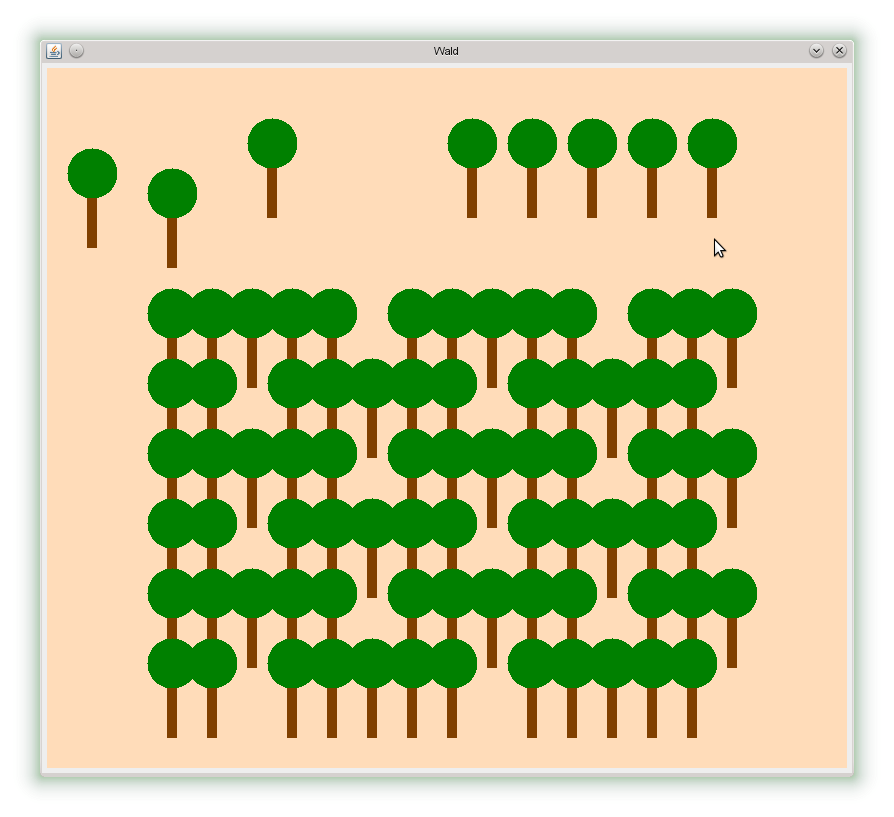
\includegraphics[width=0.8\textwidth]{./inf/SEKII/09_Java_Farben_und_Zufall/Aufgabe1.png}
\end{center}


\subsection{Aufgabe 2: Wald mit Zufallspositionen}

\begin{compactenum}[a)]
\item Erzeuge eine neue Klasse für ein Anwendungsfenster mit einer Breite und
Höhe von je 500 Pixeln (dies sind die Standardwerte). Kopiere die Methode
\lstinline|baum()| aus Aufgabe 1 in die neue Klasse hinein.
\item Erzeuge in einer Schleife 50 Bäume an zufälligen Positionen. Für die
x-Position eines Baumes sollen jeweils Zufallswerte zwischen 0 und 449 erzeugt
werden. Für die y-Position eines Baumes sollen Zufallswerte zwischen 30 und 499
erzeugt werden.
\end{compactenum}


\subsection{Aufgabe 3: Diagonale}

\begin{minipage}{0.5\textwidth}
\begin{compactenum}[a)]
\item Erzeuge ein neues Anwendungsfenster mit einer Breite von 520 Pixeln und
einer Höhe von 520 Pixeln. Das Anwendungsfenster soll eine schwarze
Hintergrundfarbe erhalten.
\item Programmiere eine Diagonale von 10 grünen Quadraten (dazu kannst du die
grüne Standardfarbe nehmen), die von links unten nach rechts oben hoch geht. Die
Quadrate besitzen alle eine Breite von 50 Pixeln. Das erste Quadrat links unten
hat die Koordinaten (10,460). Zwischen den Eckpunkten der Quadrate soll sich
keine Lücke befinden.
\item Jedes einzelne Quadrat soll zufällig entweder die Farbe rot, grün oder
gelb erhalten (dazu kannst du die Standardfarben verwenden). Erzeuge dazu für
jedes Quadrat eine Zufallszahl zwischen 0 und 2 und setze die Zahl dann mit
einer \lstinline|switch|-Anweisung in einen Zufallswert um.
\end{compactenum}
\end{minipage}\hfill
\begin{minipage}{0.45\textwidth}
\centering
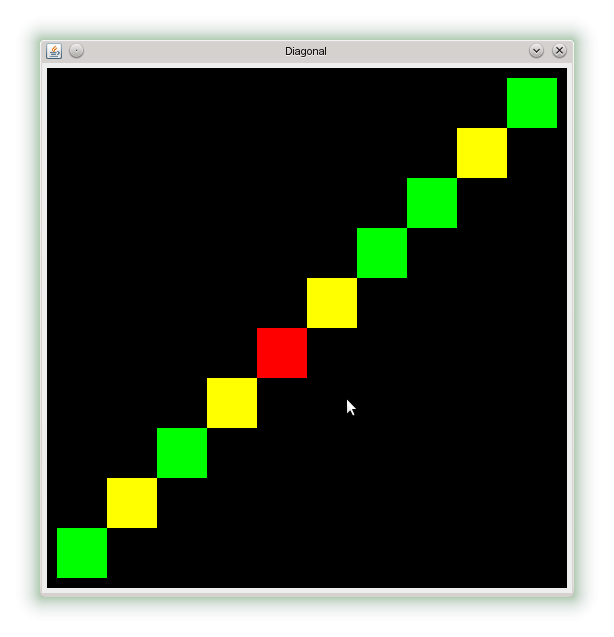
\includegraphics[width=1.0\textwidth]{./inf/SEKII/09_Java_Farben_und_Zufall/Aufgabe3.png}
\end{minipage}


\subsection{Aufgabe 4: Farbsäule}

Erstelle ein neues Anwendungsfenster mit einer schwarzen Hintergrundfarbe.

Zeichne in dem Anwendungsfenster eine Säule mit acht untereinander liegenden
Rechtecken, die alle einen anderen Rot-Ton erhalten. Das oberste Quadrat erhält
ein tiefes dunkelrot, dass folgendermaßen gemischt wird:

\begin{lstlisting}
Color rot = new Color(50,0,0);
\end{lstlisting}

Bei den nachfolgenden Rechtecken wird der Rot-Anteil der Farbe jeweils um 25
erhöht, so dass die Rechtecke immer heller und heller werden.

Jedes Rechteck soll eine Breite von 100 Pixeln und eine Höhe von 50 Pixeln
besitzen. Alle Rechtecke liegen ohne Lücke direkt untereinander. Das oberste
Rechteck hat die Position (200,70).